\documentclass[11pt,a4paper]{article}

\usepackage[utf8]{inputenc}
\usepackage[T1]{fontenc}
\usepackage[spanish,es-nodecimaldot,es-noquoting]{babel}

% ==============================================================================
% Preamble of the PCB application note (Spanish).
% Loaded by main_es.tex and main_en.tex after they load babel.
% Only standard packages, and no \spanishdeactivate: it breaks local builds.
% ==============================================================================

\usepackage[margin=2.2cm, headheight=15pt]{geometry}
\usepackage{lmodern}
\usepackage{microtype}
\usepackage{amsmath}
\usepackage{graphicx}
\usepackage{float}
\usepackage{caption}
\usepackage{xcolor}
\usepackage{colortbl}
\usepackage{array}
\usepackage{tabularx}
\usepackage{booktabs}
\usepackage{longtable}
\usepackage{enumitem}
\usepackage{fancyhdr}
\usepackage{tikz}
\usetikzlibrary{arrows.meta,positioning,babel}
\usepackage[hidelinks]{hyperref}
\usepackage{xurl}
\urlstyle{tt}
% File paths and names: they break at slashes and underscores.
\newcommand{\ruta}[1]{\nolinkurl{#1}}
\setlength{\emergencystretch}{2em}

\definecolor{headbg}{HTML}{DCE6F1}
\definecolor{groupbg}{HTML}{F2F2F2}

% Table with a shaded header row.
\newcommand{\tablehead}[1]{\rowcolor{headbg}#1}

\setlist{itemsep=2pt, topsep=4pt}
\setlength{\parindent}{0pt}
\setlength{\parskip}{6pt}
\renewcommand{\arraystretch}{1.15}

\pagestyle{fancy}
\fancyhf{}
\fancyhead[L]{\small DR-VF-01 -- Nota de aplicación de la PCB}
\fancyhead[R]{\small \reportrevision}
\fancyfoot[C]{\small \thepage}

% Numbers and facts that appear in the text come from one file, for both languages.
% ==============================================================================
% Every number of the note comes from this file. evidence/check_numbers.py
% recomputes each one from its source and fails if they differ.
% Macro names contain letters only (TeX does not allow digits in them).
% ==============================================================================

\newcommand{\reportrevision}{Rev. 1.0}

% --- Board (from hardware/pcb/DR-VF-01_gerbers.zip, BOM CSV and DRC summary) ---
\newcommand{\bBoardWidth}{64.4}        % mm, Gerber profile PCB.GM
\newcommand{\bBoardHeight}{88.8}       % mm, Gerber profile PCB.GM
\newcommand{\bLayers}{2}
\newcommand{\bThickness}{0.8}          % mm, docs/ARCHITECTURE.md 5.2
\newcommand{\bParts}{112}              % placed parts, BOM CSV
\newcommand{\bBomLines}{54}            % BOM CSV lines
\newcommand{\bHoles}{185}              % drill report PCB.DRR
\newcommand{\bViaHoles}{160}           % 0.305 mm plated holes, PCB.DRR
\newcommand{\bDrcRules}{31}            % evidence/drc_summary.txt
\newcommand{\bDrcViolations}{0}

% --- Design rules loaded in Altium (evidence/drc_summary.txt) ---
\newcommand{\rClearance}{0.152}        % mm
\newcommand{\rViaHole}{0.305}          % mm
\newcommand{\rViaDiameter}{0.61}       % mm
\newcommand{\rRfWidth}{1.346}          % mm, preferred width of class RF50
\newcommand{\rUsbWidth}{0.254}         % mm, preferred width of class USB
\newcommand{\rPwrWidth}{0.406}         % mm, preferred width of class PWR
\newcommand{\rChargerWidth}{0.508}     % mm, preferred width of class PWR_CN3791

% --- the same lengths in mil (1 mil = 0.0254 mm), as Altium shows them; check_numbers.py compares them with the mm values ---
\newcommand{\mBoardWidth}{2535}
\newcommand{\mBoardHeight}{3496}
\newcommand{\mThickness}{31.5}
\newcommand{\mClearance}{6}
\newcommand{\mViaHole}{12}
\newcommand{\mViaDiameter}{24}
\newcommand{\mRfWidth}{53}
\newcommand{\mUsbWidth}{10}
\newcommand{\mPwrWidth}{16}
\newcommand{\mChargerWidth}{20}
\newcommand{\mRestWidth}{8}

% --- Design values as drawn in the schematic (hardware/pcb/DR-VF-01_schematics.pdf, sheet 1)
%     and calculations that use them. docs/ARCHITECTURE.md still shows older values for the
%     MPPT divider (402 k / 100 k) and the sense resistor (0.12 ohm); the schematic wins.
\newcommand{\cVin}{6.0}                % V, solar panel
\newcommand{\cVbat}{4.2}               % V, full battery
\newcommand{\cFsw}{300}                % kHz, CN3791 switching frequency
\newcommand{\cLused}{47}               % uH, L1 (CY54-47UH)
\newcommand{\cLmin}{25}                % uH, datasheet rule L > 5 (Vcc - Vbat) with Vcc = 8 V, Vbat = 3 V
\newcommand{\cRtop}{400}               % kohm, R8 390 k + R9 10 k
\newcommand{\cRbottom}{100}            % kohm, R10
\newcommand{\cVmppt}{6.03}             % V
\newcommand{\cVstart}{6.15}            % V
\newcommand{\cRcs}{0.47}               % ohm, R12
\newcommand{\cIcs}{255}                % mA, 120 mV / 0.47 ohm
\newcommand{\cRipple}{89}              % mA, inductor ripple with 47 uH
\newcommand{\cRipplePct}{35}           % % of the charge current
\newcommand{\cRprog}{1.9}              % kohm, R5 1.8 k + R6 100 ohm
\newcommand{\cIcharge}{480}            % mA, scaled from the TP4056 datasheet (0.91 k -> 1 A)
\newcommand{\cPtp}{0.65}               % W, (5 - 3.7) V x 0.5 A, current limit of the design document
\newcommand{\cPldo}{0.27}              % W
\newcommand{\cIsleep}{124}             % uA (123.76)
\newcommand{\cIactive}{88}             % mA
\newcommand{\cIpeak}{224}              % mA
\newcommand{\cIlimit}{150}             % uA, RNF-03
\newcommand{\cMargin}{26}              % uA
\newcommand{\cDays}{190}               % days, POWER_BUDGET.md profile (0.223 mA average), 1020 mAh effective
\newcommand{\cCapEff}{1020}            % mAh, 1200 x 0.85
\newcommand{\cIdoc}{0.223}             % mA, average current of the POWER_BUDGET.md profile
\newcommand{\cIfsm}{1.06}              % mA, average current of the FSM-consistent profile (docs/design-reviews/power.md PH-2)
\newcommand{\cDaysLow}{40}             % days, FSM-consistent profile
\newcommand{\cDaysSleep}{343}          % days, sleep only at 123.76 uA (upper bound, not a real autonomy)
\newcommand{\cEnergySeven}{177}        % mAh used by 7 dark days (25.3 mAh/day, PH-2)

% --- Thingy:91 X measurements (copied from ../engineering_report_poc/data.tex) ---
\newcommand{\pSoc}{nRF9151}
\newcommand{\pBoard}{Nordic Thingy:91\,X}
\newcommand{\pBenchUsFour}{350.2}
\newcommand{\pBenchMsThousand}{61.42}
\newcommand{\pBenchLimitVertices}{833}
\newcommand{\pCepLow}{3.46}
\newcommand{\pCepHigh}{7.35}
\newcommand{\pReqCep}{2.5}
\newcommand{\pWalkAccMin}{2.0}
\newcommand{\pWalkAccMax}{2.6}
\newcommand{\pTtffA}{54}
\newcommand{\pTtffB}{90}
\newcommand{\pTtffC}{136}
\newcommand{\pFlashBytes}{94\,268}
\newcommand{\pRamBytes}{19\,776}


\graphicspath{{../../hardware/pcb/}}

\title{\textbf{Collar DR-VF-01\\Nota de aplicación: PCB de la cerca virtual con ESP32-S3}}
\author{Universidad Nacional de Colombia\\Departamento de Ingeniería Eléctrica, Electrónica y Computación (DIEEC)}
\date{\today}

\begin{document}

\maketitle
\thispagestyle{empty}
\tableofcontents
\clearpage

\section{Acerca de este documento}

\subsection{Alcance y propósito}

Esta nota de aplicación describe la PCB del collar DR-VF-01, diseñada en Altium Designer: qué
hace cada bloque, cómo se calcularon sus valores, cómo se dispusieron las pistas y qué se verificó.
Sigue el formato de los diseños de referencia de los fabricantes de semiconductores (especificaciones
clave, diagrama de bloques, teoría de diseño, resultados y archivos de diseño), para que un ingeniero
pueda entender el diseño, revisarlo y reproducirlo.

La placa está \textbf{diseñada y no fabricada}: pasó la verificación de reglas de diseño (DRC) de
Altium sin violaciones, pero ninguna cifra eléctrica o de radiofrecuencia se ha medido en una placa
real. Por eso la nota distingue siempre entre lo que se cumple \emph{por diseño} (cálculo, esquemático o
DRC), lo que se midió en otra plataforma y lo que queda pendiente de medir cuando exista la placa.

El producto completo, con sus requerimientos, su arquitectura y su análisis comercial, está en la
\emph{Memoria Técnica} (\ruta{docs/DR-VF-01_Memoria_Tecnica.pdf}), a la que esta nota remite y
que no repite. La prueba de concepto del firmware sobre la \pBoard{} tiene su propio informe en
\ruta{docs/poc-thingy91x/}.

\subsection{Público}

Ingenieros de hardware o de firmware que revisen o continúen el diseño, y quien evalúe el proyecto.

\subsection{Datos de la placa}

\begin{table}[H]
\centering
\small
\begin{tabularx}{\textwidth}{|l X|}
\hline
\tablehead{\textbf{Elemento} & \textbf{Valor}} \\ \hline
Herramienta & Altium Designer 26.11.1 \\ \hline
Contorno & \mBoardWidth{} $\times$ \mBoardHeight~mil (\bBoardWidth{} $\times$ \bBoardHeight~mm, perfil de los Gerbers) \\ \hline
Capas y material & \bLayers{} capas de cobre, FR4 de \mThickness~mil \\ \hline
Fabricante previsto & JLCPCB, acabado ENIG (decisión del 2026-11-07, \ruta{hardware/PCB_REGLAS.md}) \\ \hline
Piezas colocadas & \bParts{} en \bBomLines{} líneas del BOM \\ \hline
Agujeros & \bHoles{} (de ellos \bViaHoles{} de \mViaHole~mil, vías y pads pasantes) \\ \hline
Verificación DRC & \bDrcRules{} reglas, \bDrcViolations{} violaciones (2026-11-15) \\ \hline
Estado & Diseñada, no fabricada \\ \hline
\end{tabularx}
\caption{Datos de la PCB.}
\end{table}

\subsection{Historial de revisiones}

\begin{table}[H]
\centering
\small
\begin{tabularx}{\textwidth}{|c l X|}
\hline
\tablehead{\textbf{Rev.} & \textbf{Estado} & \textbf{Contenido}} \\ \hline
0.9 & Borrador & Estructura y contenido completos. Incluye las vistas 3D de la placa. Falta el reporte ERC y la decisión sobre los hallazgos del BOM; los dos de RF tienen decisión (2026-11-26). \\ \hline
1.0 & Planeada & Versión de entrega, con las figuras de la placa y las decisiones tomadas. \\ \hline
\end{tabularx}
\caption{Revisiones de la nota.}
\end{table}

\section{Especificaciones clave}

La tabla siguiente reproduce los requerimientos de la Memoria Técnica
(\ruta{docs/REQUIREMENTS.md}, versión vigente). Es la única fuente de requerimientos: esta nota no
añade ninguno. La tabla de cumplimiento (sección~\ref{sec:cumplimiento}) vuelve a esta lista y dice,
para cada uno, qué se cumple y con qué evidencia. Las frases entre comillas son el texto original; el
texto completo, con la trazabilidad, está en el archivo citado.

\begin{longtable}{|p{1.4cm} p{5.2cm} p{8.5cm}|}
\caption{Requerimientos funcionales (RF) y no funcionales (RNF) de la Memoria Técnica.}\\
\hline
\tablehead{\textbf{ID} & \textbf{Descripción} & \textbf{Métrica o criterio de aceptación}} \\ \hline
\endfirsthead
\hline
\tablehead{\textbf{ID} & \textbf{Descripción} & \textbf{Métrica o criterio de aceptación}} \\ \hline
\endhead
RF-01 & Geolocalización mediante GNSS multiconstelación & Error de posición $<$ 2.5~m (métrica por definir: CEP o RMS) \\ \hline
RF-02 & Evaluación de cerca virtual (algoritmo Point-in-Polygon) & Tiempo de procesamiento $<$ 50~ms \\ \hline
RF-03 & Acción disuasiva simulada con optoacoplador & Activación de LED indicador al cruzar geocerca \\ \hline
RF-04 & Telemetría LoRa en banda 915~MHz & Envío de paquetes formateados (Lat, Lon, Battery \%, Satellites, Fence Status) \\ \hline
RF-05 & Monitoreo de porcentaje de batería & Lectura vía bus I2C con actualización constante \\ \hline
RF-06 & Despertar desde Deep Sleep por movimiento (\emph{wake-on-motion}) & Por definir (sin métrica aprobada) \\ \hline
RF-07 & Actualización remota de la geocerca por red celular (propuesto el 2026-11-25, sin aprobar) & Una cerca dibujada en el portal llega al collar, se valida, se guarda en flash y se aplica; latencia máxima igual al intervalo de consulta más 30~s (propuesta); una cerca inválida se rechaza y se informa \\ \hline
RNF-01 & Autonomía energética con panel solar de 6~V, de 1 a 1.5~W & 7 días de operación en oscuridad total con batería de 1200~mAh \\ \hline
RNF-02 & Procesamiento determinista en Zephyr RTOS & Ejecución sin bloqueo de tareas críticas \\ \hline
RNF-03 & Consumo en estado Deep Sleep & $<$ 150~\textmu A total del circuito \\ \hline
RNF-04 & Fiabilidad mecánica sin cables de puente & PCB final sin jumpers o falsos contactos \\ \hline
RNF-05 & Carga por USB-C & 500~mA de corriente de carga (RPROG de 1.9~k$\Omega$); no menos de 3~h para 1500~mAh (2.4~h para 1200~mAh) antes de la cola a tensión constante \\ \hline
RNF-06 & Protección de la batería & Por definir (sin métrica aprobada) \\ \hline
RNF-07 & Protección ESD en el puerto USB-C & Por definir (sin métrica aprobada) \\ \hline
RNF-08 & Protección IP67 de la carcasa & IP67 (objetivo de diseño) \\ \hline
RNF-09 & Rango de temperatura de operación & 0 a $+65$~\textdegree C, límite ambiente del módulo dentro de la carcasa \\ \hline
\end{longtable}

Tres requerimientos nombran piezas concretas: RF-01 el receptor u-blox MAX-M10S, RF-02 el
microcontrolador ESP32-S3 y RF-04 el módulo LoRa DX-LR30-900M22S. La PCB las usa; la prueba de
concepto del firmware usó otra plataforma, con otro receptor GNSS y otro procesador, y sus resultados
solo sirven aquí como referencia indicativa (sección~\ref{sec:verificacion}).

\section{Diagrama de bloques y componentes}

\subsection{Cómo está organizada la placa}

La batería es el nodo central. Dos cargadores independientes la cargan, uno desde el panel solar
(CN3791) y otro desde el USB-C (TP4056), y todo el sistema se alimenta de ella a través de un
regulador lineal de 3.3~V. El USB-C no alimenta al sistema: solo carga la batería y lleva los datos
de programación. Por eso, sin batería conectada la placa no arranca desde el USB.

\begin{figure}[H]
\centering
\resizebox{0.97\textwidth}{!}{%
\begin{tikzpicture}[
  box/.style={draw, rounded corners, align=center, font=\scriptsize, minimum height=0.9cm, text width=2.6cm},
  src/.style={box, fill=groupbg},
  core/.style={box, fill=headbg},
  >=Stealth]
\node[src] (sol) at (-6.2,2.2) {Panel solar\\6~V};
\node[src] (usb) at (-6.2,0.2) {USB-C\\5~V (y datos)};
\node[box] (cn) at (-3.1,2.2) {Cargador solar\\CN3791 (U3)};
\node[box] (tp) at (-3.1,0.2) {Cargador USB\\TP4056 (U2)};
\node[core] (bat) at (0,1.2) {Batería 1S\\3.7~V, con protección\\integrada};
\node[box] (ldo) at (3.1,1.2) {LDO 3.3~V\\TLV75733P (U4)};
\node[box] (gau) at (0,-0.9) {Medidor de batería\\MAX17048 (U9)};
\node[core] (mcu) at (7.0,3.0) {ESP32-S3\\WROOM-1U (U5)};
\node[box] (gps) at (7.0,1.8) {GNSS\\MAX-M10S (U6)};
\node[box] (lor) at (7.0,0.6) {LoRa\\DX-LR30 (U7)};
\node[box] (imu) at (7.0,-0.6) {IMU\\LSM6DS3TR-C (U8)};
\draw[->] (sol) -- (cn); \draw[->] (usb) -- (tp);
\draw[->] (cn) -- (bat); \draw[->] (tp) -- (bat);
\draw[->] (bat) -- (ldo); \draw[->] (bat) -- (gau);
\draw[->] (ldo.east) -- ++(0.35,0) |- (mcu.west);
\draw[->] (ldo.east) -- ++(0.35,0) |- (gps.west);
\draw[->] (ldo.east) -- ++(0.35,0) |- (lor.west);
\draw[->] (ldo.east) -- ++(0.35,0) |- (imu.west);
\end{tikzpicture}}
\caption{Diagrama de bloques de la alimentación y de los módulos de la PCB.}
\end{figure}

\subsection{Componentes principales}

\begin{table}[H]
\centering
\footnotesize
\begin{tabularx}{\textwidth}{|l l X|}
\hline
\tablehead{\textbf{Ref.} & \textbf{Pieza} & \textbf{Función}} \\ \hline
U5 & ESP32-S3-WROOM-1U-N16R8 & Procesador de la aplicación (Zephyr); versión con conector u.FL, sin antena impresa \\ \hline
U6 & u-blox MAX-M10S-00B & Receptor GNSS multiconstelación en L1, por UART; parche pasivo con cable y u.FL (J4) \\ \hline
U7 & DX-LR30-900M22S & Módulo LoRa con SX1262, 915~MHz, por SPI; antena de 8~cm por u.FL (J5) \\ \hline
U8 & LSM6DS3TR-C & IMU; su interrupción despierta al MCU del sueño profundo \\ \hline
U9 & MAX17048G+T10 & Medidor de carga de la batería por I2C (0x36), conectado a la batería \\ \hline
U3 & CN3791 & Cargador solar conmutado con seguimiento de punto de máxima potencia (MPPT), con L1 de 47~\textmu H \\ \hline
U2 & TP4056 & Cargador lineal desde USB-C, limitado a 500~mA \\ \hline
U4 & TLV75733PDBVR & LDO de 3.3~V, 1~A, corriente en reposo de 25~\textmu A, alimentado solo desde la batería \\ \hline
U1 & USBLC6-2SC6 & Protección ESD en D+, D$-$ y VBUS del USB-C (J1) \\ \hline
U10 & VO617A-1X017T & Optoacoplador: aislamiento galvánico del actuador \\ \hline
D3, D4, BZ1 & LED RGB, LED rojo, zumbador PS1240P02BT & Alertas visuales y sonora \\ \hline
Y1 & ECS-.327-12.5-34B-TR & Cristal de 32.768~kHz \\ \hline
\end{tabularx}
\caption{Componentes principales y su designador en el esquemático.}
\end{table}

\subsection{Hojas del esquemático}

El esquemático tiene cinco hojas: potencia y carga, microcontrolador, radio (GNSS y LoRa), sensores
(IMU y medidor de batería) e interfaz (optoacoplador, LEDs, zumbador y botón). Las páginas están en
\ruta{hardware/pcb/DR-VF-01_schematics.pdf} y se reproducen a continuación.

\foreach \p in {1,...,5}{%
\begin{figure}[p]
\centering
\includegraphics[width=\textwidth,page=\p]{DR-VF-01_schematics.pdf}
\caption{Hoja \p{} del esquemático.}
\end{figure}}

\section{Teoría de diseño}

Los valores de esta sección están calculados en \ruta{docs/ARCHITECTURE.md} y
\ruta{hardware/POWER_BUDGET.md}; aquí se repiten los pasos para que se puedan revisar. Ninguno se
ha medido en una placa.

\subsection{Cargador solar CN3791}

Los valores de esta subsección son los del esquemático (hoja 1, bloques 1B y 1C).

\textbf{Corriente de carga.} La corriente la fija la resistencia de sensado R12, de \cRcs~$\Omega$, con la
referencia interna de 120~mV del CN3791:
\[
I_{CH} = \frac{120~\text{mV}}{R_{CS}} = \frac{0.12~\text{V}}{\cRcs~\Omega} \approx \cIcs~\text{mA}.
\]
Es una corriente moderada, acorde con un panel de 6~V de entre 1 y 1.5~W (unos 250~mA como máximo).

\textbf{Inductancia.} Con la bobina L1 de \cLused~\textmu H (CY54-47UH, 0.71~A, del docente), el rizado de
corriente en el peor caso (entrada de \cVin~V, batería de \cVbat~V, \cFsw~kHz) es:
\[
\Delta I_L = \frac{V_{BAT}\,(V_{IN}-V_{BAT})}{V_{IN}\,f_{sw}\,L}
  = \frac{4.2\,(6.0-4.2)}{6.0\cdot 300\,000\cdot 47\cdot 10^{-6}} \approx \cRipple~\text{mA},
\]
es decir, un \cRipplePct~\% de la corriente de carga. El datasheet del CN3791 exige además
$L > 5\,(V_{CC}-V_{BAT})~\mu\text{H}$: con el panel en circuito abierto (unos 8~V) y la batería a 3.0~V
resultan más de \cLmin~\textmu H, que \cLused~\textmu H cumple y 10~\textmu H no.

\textbf{Punto de trabajo del panel (MPPT).} El pin MPPT se regula a 1.205~V. El divisor lleva
R8 (390~k$\Omega$) y R9 (10~k$\Omega$) en serie hacia el panel y R10 (100~k$\Omega$) a masa, de modo que
la tensión a la que trabaja el panel es:
\[
V_{MPPT} = 1.205\left(1+\frac{R_8+R_9}{R_{10}}\right) = 1.205\left(1+\frac{\cRtop}{\cRbottom}\right) \approx \cVmppt~\text{V}.
\]
El ciclo de carga solo empieza cuando el pin MPPT supera 1.23~V, es decir, con más de
$1.23\cdot 5 \approx \cVstart$~V en la entrada. Por eso un USB de 5~V nunca arranca este cargador, y la
carga por USB va por otro circuito integrado. Un transistor N (Q3), gobernado por la señal
\ruta{CHG_INHIBIT} del MCU, baja el pin MPPT para inhibir la carga solar.

\subsection{Cargador USB TP4056}

Con $R_{PROG} = \cRprog$~k$\Omega$ (R5 de 1.8~k$\Omega$ más R6 de 100~$\Omega$) la corriente queda en unos \cIcharge~mA, escalando el dato del datasheet del fabricante (0.91~k$\Omega$ da 1~A); el diseño la documenta como 500~mA. Es un cargador lineal, así que
disipa la diferencia de tensión por la corriente: con 5~V de entrada, la celda a 3.7~V y los 500~mA del documento de diseño,
$(5-3.7)\cdot 0.5 = \cPtp$~W. Su regulación térmica protege el chip a 145~\textdegree C, y el pad
térmico va a una zona amplia de cobre de masa. A 500~mA, la carga tarda no menos de 3~h para
1500~mAh.

\subsection{Regulador de 3.3~V}

El TLV75733P recibe como máximo 4.2~V de la batería. Con una carga de 300~mA disipa
$(4.2-3.3)\cdot 0.3 = \cPldo$~W, dentro de lo que admite su encapsulado con cobre y vías térmicas.
Se descartó el DS8570F8 del docente porque consume 0.6~mA con la salida activa y sin carga, 24 veces
los 25~\textmu A del TLV75733P.

\subsection{Presupuesto de consumo}

\begin{table}[H]
\centering
\footnotesize
\begin{tabularx}{\textwidth}{|l l l l X|}
\hline
\tablehead{\textbf{Módulo} & \textbf{Reposo} & \textbf{Activo} & \textbf{Pico} & \textbf{Observaciones}} \\ \hline
ESP32-S3 & 8~\textmu A & 70~mA & 240~mA & Wi-Fi solo en modo de configuración \\ \hline
MAX-M10S & 46~\textmu A & 12~mA & 35~mA & Reposo por software \\ \hline
DX-LR30 (SX1262) & 0.6~\textmu A & 5.3~mA & 118~mA & Ráfagas de fracciones de segundo; valores del chip \\ \hline
IMU & 9.5~\textmu A & 0.55~mA & 1~mA & Valores presupuestados \\ \hline
MAX17048 & 3~\textmu A & 0.023~mA & 0.05~mA & Hibernación \\ \hline
CN3791 & 30~\textmu A & --- & --- & Sin entrada, desde la batería \\ \hline
TLV75733P & 25~\textmu A & --- & --- & Corriente en reposo \\ \hline
TP4056 & 2.5~\textmu A & --- & --- & En espera \\ \hline
\textbf{Total} & \textbf{$\approx$ \cIsleep~\textmu A} & \textbf{$\approx$ \cIactive~mA} & \textbf{$\approx$ \cIpeak~mA} & Calculado; ver los pendientes \\ \hline
\end{tabularx}
\caption{Consumo por módulo y total del sistema (\ruta{hardware/POWER_BUDGET.md}).}
\end{table}

El consumo en sueño profundo calculado, de unos \cIsleep~\textmu A, deja un margen de \cMargin~\textmu A
frente al límite de \cIlimit~\textmu A de RNF-03. El margen es estrecho: faltan por sumar el USBLC6-2SC6,
la fuga de los dos diodos Schottky del CN3791, que debe quedar por debajo de unos 47~\textmu A en total, y
los consumos extra del módulo LoRa. Los valores son típicos; el consumo real solo se sabrá midiendo la
primera placa. Con una batería de 1200~mAh, la autonomía estimada en oscuridad es de unos \cDays~días.

\section{Diseño de la PCB}

\subsection{Apilado y contorno}

La placa tiene \bLayers{} capas de cobre sobre FR4 de \bThickness~mm (el espesor del diseño
recomendado del conector USB-C de 16 pines), con un contorno de \bBoardWidth{} $\times$
\bBoardHeight~mm. La capa inferior lleva un vertido de masa continuo, que sirve de plano de
referencia de las líneas de radiofrecuencia y del USB. Al ser de dos capas, el fabricante no ofrece
impedancia controlada, y el diseño acepta esa dispersión en líneas cortas.

\subsection{Clases de red y reglas cargadas en Altium}

\begin{table}[H]
\centering
\footnotesize
\begin{tabularx}{\textwidth}{|l l X|}
\hline
\tablehead{\textbf{Clase} & \textbf{Ancho preferido} & \textbf{Uso}} \\ \hline
\texttt{RF50} & \rRfWidth~mm & Línea de 50~$\Omega$ del LoRa y del GNSS hasta sus conectores u.FL, microstrip sobre el plano de la capa inferior \\ \hline
\texttt{USB} & \rUsbWidth~mm & Par diferencial D+/D$-$, con longitudes igualadas \\ \hline
\ruta{PWR_CN3791} & \rChargerWidth~mm & Lazo del cargador solar (diodos, MOSFET, bobina) \\ \hline
\texttt{PWR} & \rPwrWidth~mm & 3V3, batería y alimentación en general \\ \hline
Resto & 0.203~mm & Señales \\ \hline
\end{tabularx}
\caption{Clases de red y ancho de pista preferido.}
\end{table}

Reglas generales: separación mínima entre cobre de \rClearance~mm, vías con agujero de \rViaHole~mm y
diámetro de \rViaDiameter~mm, y separaciones propias del componente USB-C y del U8. El ancho de la línea de
50~$\Omega$ salió de un cálculo de microstrip sobre FR4 de \bThickness~mm con $\varepsilon_r = 4.4$
(estimación, \ruta{hardware/PCB_REGLAS.md}): con la tolerancia de espesor del fabricante queda entre
unos 46 y 54~$\Omega$.

\subsection{Criterios de ubicación}

Los criterios de zonificación salen de las guías de integración de u-blox y de Espressif
(\ruta{hardware/PCB_REGLAS.md}):
\begin{itemize}
  \item los componentes de radiofrecuencia del GNSS, a 5~mm como mínimo de cualquier otro componente de RF y lejos de lo digital;
  \item el parche GNSS y su conector, del lado opuesto al Wi-Fi del módulo y al LoRa;
  \item el MAX-M10S, lejos de fuentes de calor (TP4056, CN3791, bobina) y sin pistas de otras señales debajo del módulo;
  \item el lazo del CN3791 lo más corto posible, y su etapa de potencia lo más lejos posible del GNSS y del cristal;
  \item el pad térmico del TP4056 a masa con una zona amplia de cobre y vías hacia la capa inferior.
\end{itemize}
Que el layout final cumpla cada criterio no se ha auditado para esta nota; es un punto de la revisión
de la placa antes de fabricarla (sección~\ref{sec:limitaciones}).

\subsection{Verificación de reglas de diseño}

El DRC de Altium del 15 de noviembre de 2026 comprobó \bDrcRules{} reglas y detectó \bDrcViolations{}
violaciones, sin ninguna excepción concedida. Entre ellas: separación de cobre, cortocircuitos, nets sin
rutear, anchos por clase, vías, anillo mínimo, separación entre agujeros, lengüetas de máscara, serigrafía,
longitudes igualadas del par USB y separaciones entre componentes. El resumen de cada regla está en
\ruta{evidence/drc_summary.txt}. El DRC verifica las reglas que se cargaron, no el diseño completo: no
sustituye a la revisión de integridad de señal ni a la de radiofrecuencia.

\subsection{Taladros}

\begin{table}[H]
\centering
\small
\begin{tabular}{|l l r l|}
\hline
\tablehead{\textbf{Herramienta} & \textbf{Diámetro} & \textbf{Cantidad} & \textbf{Tipo}} \\ \hline
T1 & 0.305~mm & 160 & Pasante metalizado \\ \hline
T2 & 0.381~mm & 11 & Pasante metalizado \\ \hline
T3 & 0.6~mm & 4 & Ranura metalizada \\ \hline
T4 & 0.762~mm & 4 & Pasante metalizado \\ \hline
T5 & 0.8~mm & 2 & Pasante metalizado \\ \hline
T6 & 0.85~mm & 2 & Pasante metalizado \\ \hline
T7 & 0.65~mm & 2 & No metalizado \\ \hline
\end{tabular}
\caption{Taladros de la placa (informe de taladro de Altium); \bHoles{} en total.}
\end{table}

\section{Firmware y portabilidad}

El firmware es un único código base sobre Zephyr RTOS para dos placas: la prueba de concepto en la
\pBoard{} y el producto final en esta PCB. Se comparten el motor de geocerca (\ruta{geofence.c}, en C puro y
sin dependencia del SDK), la máquina de estados y el registro de eventos. Cada placa aporta su archivo de
overlay del árbol de dispositivos, su \ruta{prj.conf} y los adaptadores de GNSS, comunicaciones e IMU.

\subsection{Qué cambia entre las dos placas}

\begin{table}[H]
\centering
\footnotesize
\begin{tabularx}{\textwidth}{|l X X|}
\hline
\tablehead{\textbf{Aspecto} & \textbf{\pBoard{} (\pSoc)} & \textbf{PCB (ESP32-S3)}} \\ \hline
GNSS & Receptor dentro del firmware del módem, con la biblioteca \ruta{nrf_modem}; sin UART ni NMEA & MAX-M10S por UART1 (GPIO17 y 18), tramas NMEA o UBX; es otro \emph{backend} del mismo adaptador \\ \hline
Comunicaciones & LTE-M y NB-IoT (no usadas en la PoC) & LoRa SX1262 por SPI (GPIO10 a 13, con BUSY, DIO1, NRESET, RXEN y TXEN) \\ \hline
Movimiento y energía & No se usan & IMU por I2C con su interrupción en GPIO4; MAX17048 por I2C (GPIO8 y 9) \\ \hline
Actuadores & LED RGB de la placa & Optoacoplador (GPIO1), zumbador (GPIO2), LED RGB (GPIO38 a 40) \\ \hline
Carga y arranque & MCUboot, imagen por USB-C & USB nativo (GPIO19 y 20), botón BOOT a masa \\ \hline
Lo que se reutiliza & \multicolumn{2}{>{\raggedright\arraybackslash}X|}{\ruta{geofence.c}, la máquina de estados, la lógica de alerta, el registro y la estructura de adaptadores} \\ \hline
\end{tabularx}
\caption{Diferencias entre las dos plataformas; el mapa de pines vigente es \ruta{hardware/pinout.md}.}
\end{table}

\subsection{Lo que validó la prueba de concepto}

En la \pBoard{} se ejecutó el motor de geocerca, la máquina de estados y la alerta con un receptor GNSS
real, y los módulos de C puro se probaron en el PC (miles de casos aleatorios, sin fallos). Seis de esos
módulos compilan sin cambios para Cortex-M33 y para ESP32-S3, con advertencias como errores, pero
\textbf{nada se ha ejecutado en el ESP32-S3}: la adaptación al MAX-M10S, a LoRa, a la IMU y al sueño
profundo existe solo como diseño en \ruta{docs/firmware_docs/}. El informe de la prueba de concepto
(\ruta{docs/poc-thingy91x/}) detalla el método y los resultados.

\section{Resultados de verificación}
\label{sec:verificacion}

Cada resultado indica qué plataforma lo produjo. Ninguna medición eléctrica o de radio de esta sección
se hizo en la PCB, que no está fabricada.

\subsection{Sobre la PCB: verificación por diseño}

\begin{table}[H]
\centering
\footnotesize
\begin{tabularx}{\textwidth}{|l X X|}
\hline
\tablehead{\textbf{Verificación} & \textbf{Resultado} & \textbf{Evidencia}} \\ \hline
DRC de Altium & \bDrcRules{} reglas, \bDrcViolations{} violaciones (2026-11-15) & \ruta{evidence/drc_summary.txt} \\ \hline
Cálculos de potencia y carga & L, divisor MPPT, $R_{CS}$, TP4056, LDO y consumo (sección~3) & \ruta{docs/ARCHITECTURE.md} \\ \hline
Presupuesto de consumo en sueño & $\approx$ \cIsleep~\textmu A frente a \cIlimit~\textmu A, con pendientes & \ruta{hardware/POWER_BUDGET.md} \\ \hline
Salidas de fabricación & Gerbers, taladros, BOM y planos generados el 2026-11-18 & \ruta{hardware/pcb/} \\ \hline
Reporte ERC de Altium & 0 errores (informe del autor, 2026-11-26) & Informe de Altium, no incluido en el repositorio \\ \hline
\end{tabularx}
\caption{Verificaciones hechas sobre el diseño de la PCB.}
\end{table}

\subsection{Referencia indicativa: medidas en la \pBoard{}}

Estos números vienen de la prueba de concepto y valen \emph{solo} para esa plataforma y esas condiciones. No
describen la PCB, que usa otro procesador, otro receptor GNSS (con más constelaciones) y otra antena.

\begin{table}[H]
\centering
\footnotesize
\begin{tabularx}{\textwidth}{|X X|}
\hline
\tablehead{\textbf{Medida en la \pBoard{} (\pSoc)} & \textbf{Valor}} \\ \hline
\ruta{geofence_check()} con 4 vértices & \pBenchUsFour~\textmu s \\ \hline
\ruta{geofence_check()} con 1024 vértices & \pBenchMsThousand~ms; llega a 50~ms cerca de los \pBenchLimitVertices{} vértices \\ \hline
Dispersión horizontal, CEP50 (cielo parcial, menos de 15 min) & \pCepLow{} a \pCepHigh~m, frente a \pReqCep~m de RF-01 \\ \hline
Exactitud estimada por el receptor al aire libre, caminando & \pWalkAccMin{} a \pWalkAccMax~m (estimación del receptor, no un CEP medido) \\ \hline
Tiempo hasta el primer fix en frío & \pTtffA, \pTtffB{} y \pTtffC~s (cronómetro manual) \\ \hline
Memoria del firmware & \pFlashBytes~B de flash y \pRamBytes~B de RAM \\ \hline
\end{tabularx}
\caption{Resultados de la prueba de concepto, a título indicativo.}
\end{table}

\section{Tabla de cumplimiento y características de diseño}
\label{sec:cumplimiento}

Esta sección es el paso de los \emph{requerimientos} a las \emph{características}. Cada fila de la
tabla de la sección~1 vuelve aquí con el valor que tiene el diseño, la evidencia y un estado. Los
estados son cinco y no se mezclan:

\begin{itemize}
  \item \textbf{Cumple por diseño}: el esquemático, un cálculo o el DRC lo respaldan; nada se midió en la placa.
  \item \textbf{Medido en PoC (otra plataforma)}: hay una medida, pero en la \pBoard{}, no en la PCB.
  \item \textbf{Pendiente de medir en la PCB}: solo se puede comprobar con la placa fabricada.
  \item \textbf{Abierto}: una revisión independiente del diseño dejó un hallazgo sin resolver que afecta al requerimiento (\ruta{docs/design-reviews/}).
  \item \textbf{Sin métrica definida}: el requerimiento no tiene criterio de aceptación aprobado.
\end{itemize}

\begin{longtable}{|p{1.5cm} >{\raggedright\arraybackslash}p{4.0cm} >{\raggedright\arraybackslash}p{3.6cm} >{\raggedright\arraybackslash}p{2.7cm} >{\raggedright\arraybackslash}p{2.2cm}|}
\caption{Cumplimiento de los requerimientos por la PCB y características de diseño.}\\
\hline
\tablehead{\textbf{ID} & \textbf{Característica del diseño} & \textbf{Evidencia} & \textbf{Estado} & \textbf{Plataforma}} \\ \hline
\endfirsthead
\hline
\tablehead{\textbf{ID} & \textbf{Característica del diseño} & \textbf{Evidencia} & \textbf{Estado} & \textbf{Plataforma}} \\ \hline
\endhead
RF-01 & MAX-M10S (U6) con parche pasivo L1 por u.FL (J4). El fabricante da 1.5~m de CEP. En la \pBoard{}, CEP50 de \pCepLow{} a \pCepHigh~m con cielo parcial, frente a \pReqCep~m & Datasheet del MAX-M10S; informe de la PoC; revisión de RF, hallazgo RF-02 (la entrada GNSS puede saturarse con los transmisores del propio collar y la placa no tiene huella para un filtro). Decisión tomada: huella de filtro SAW con puente de 0~$\Omega$ en la siguiente revisión, sin aplicar a esta PCB & Abierto; pendiente de medir en la PCB & PCB; la medida es de la PoC \\ \hline
RF-02 & \ruta{geofence_check()}: \pBenchUsFour~\textmu s con 4 vértices y \pBenchMsThousand~ms con 1024; llega a 50~ms cerca de los \pBenchLimitVertices{} vértices & Benchmark de la PoC; falta medir en el ESP32-S3 con osciloscopio & Medido en PoC (otra plataforma) & \pSoc{}, no el ESP32-S3 \\ \hline
RF-03 & Optoacoplador VO617A (U10), LED rojo (D4), LED RGB (D3) y zumbador PS1240P02BT (BZ1) en el esquemático (hoja 5) & Esquemático; el LED RGB se probó en la PoC & Cumple por diseño; pendiente de medir la corriente & PCB \\ \hline
RF-04 & DX-LR30-900M22S (U7) por SPI, antena de 8~cm por u.FL (J5) & Esquemático (hoja 3); revisión de RF, hallazgo RF-01 resuelto en los documentos: el perfil pasa de un canal fijo en 915.0~MHz, que no encajaba en ninguna categoría de uso libre en Colombia, a canales de 500~kHz dentro de 915.25 a 927.75~MHz (el firmware del LoRa aún no existe) & Cumple por diseño; confirmar con la ANE antes de pruebas de campo & PCB \\ \hline
RF-05 & MAX17048 (U9) por I2C, dirección 0x36, conectado a la batería & Esquemático (hoja 4) & Cumple por diseño; pendiente de medir contra un multímetro & PCB \\ \hline
RF-06 & Interrupción de la IMU LSM6DS3TR-C (U8) cableada a GPIO4 del ESP32-S3 & Esquemático (hojas 2 y 4) & Sin métrica definida & PCB \\ \hline
RF-07 & La PCB no tiene módem celular (ESP32-S3 con LoRa), así que el diseño no puede cumplirlo; la función existe solo en la prueba de concepto, con pruebas en el PC y compilación para la \pBoard{}, sin haberse ejecutado en la placa ni con una cuenta de nube & \ruta{docs/REQUIREMENTS.md} (RF-07, propuesto); \ruta{docs/poc-thingy91x/PRUEBAS\_LTE.md} & Sin métrica definida (propuesto, sin aprobar) & Otra plataforma; no aplica a esta PCB \\ \hline
RNF-01 & Batería de 1200~mAh sin sol: el requisito de 7 días se cumple con margen; autonomía estimada de \cDaysLow{} a \cDays~días con uso normal, y \cIsleep~\textmu A en sueño (sección~3) & \ruta{hardware/POWER_BUDGET.md}; \ruta{docs/design-reviews/power.md} (PH-2) & Cumple por diseño (estimación) & PCB \\ \hline
RNF-02 & Zephyr RTOS en ambas placas; sin traza de latencias & Informe de la PoC & Pendiente de medir en la PCB & ---\\ \hline
RNF-03 & Unos \cIsleep~\textmu A calculados frente a \cIlimit~\textmu A; margen de \cMargin~\textmu A, con consumos aún por sumar (USBLC6, diodos del CN3791, módulo LoRa) & Sección~3; \ruta{hardware/POWER_BUDGET.md} & Cumple por diseño, con margen estrecho; pendiente de medir & PCB \\ \hline
RNF-04 & Módulo ESP32-S3 soldado y conectores u.FL; sin cables de puente & Esquemático y diseño de la placa & Cumple por diseño; pendiente de inspección en la placa & PCB \\ \hline
RNF-05 & TP4056 (U2) con R5 y R6 en serie, de \cRprog~k$\Omega$ en total: unos \cIcharge~mA & Esquemático (hoja 1); datasheet del TP4056 & Cumple por diseño; pendiente de medir la corriente & PCB \\ \hline
RNF-06 & Protección de la batería integrada en la celda (PCM); la PCB no lleva circuito protector & Decisión del 2026-11-05 & Sin métrica definida & PCB \\ \hline
RNF-07 & USBLC6-2SC6 (U1) en D+, D$-$ y VBUS & Esquemático (hoja 1); faltan sus niveles ESD por verificar con el datasheet & Sin métrica definida & PCB \\ \hline
RNF-08 & Sello del conector USB-C sin definir (tipo y pieza) & \ruta{mechanical/IP67_SPEC.md} & Pendiente de medir en la PCB & Carcasa \\ \hline
RNF-09 & Módulo ESP32-S3-WROOM-1U-N16R2, de 85~\textdegree C de ambiente, en lugar del N16R8 de 65~\textdegree C; con hasta 15~\textdegree C de sol directo sobre 65~\textdegree C quedan 80~\textdegree C & Revisión del BOM, hallazgo BOM-04 (decisión del 2026-11-26); \ruta{hardware/THERMAL.md} & Cumple por diseño & PCB y carcasa \\ \hline
\end{longtable}

\subsection{Lectura de la tabla}

De las dieciséis filas, ocho se cumplen por diseño (RF-03, RF-04, RF-05, RNF-01, RNF-03, RNF-04, RNF-05 y RNF-09), una
tiene una medida en otra plataforma (RF-02), una sigue abierta por un hallazgo de las revisiones
independientes (RF-01), cuatro no tienen métrica definida (RF-06, RF-07, RNF-06 y RNF-07) y dos
esperan a la placa fabricada o a la carcasa (RNF-02 y RNF-08). Solo RF-02 tiene alguna medición, y es de
la \pBoard{}. Ningún requerimiento está \emph{verificado en la PCB}, porque la PCB aún no existe
físicamente.

\section{Limitaciones y trabajo pendiente}
\label{sec:limitaciones}

\subsection{Limitaciones de lo verificado}

\begin{itemize}
  \item \textbf{La placa no está fabricada.} Nada eléctrico ni de radiofrecuencia se ha medido: ni el consumo en sueño, ni el rizado del riel de 3.3~V al transmitir, ni la línea de 50~$\Omega$, ni el fix del GNSS con el parche, ni el alcance del LoRa, ni la enumeración por USB.
  \item \textbf{El DRC no es una revisión completa.} Comprueba las reglas cargadas. No sustituye a la revisión de integridad de señal ni a la de radiofrecuencia, y no se auditó que el layout cumpla los criterios de zonificación de la sección~4.
  \item \textbf{Los datos de la \pBoard{} son indicativos.} Otro procesador, otro receptor con menos constelaciones y otra antena. El resultado de la PoC en cielo parcial (\pCepLow{} a \pCepHigh~m de CEP50) no predice el de la PCB.
  \item \textbf{El presupuesto de consumo es calculado} con valores típicos de datasheet, con consumos todavía por sumar. El margen de \cMargin~\textmu A frente al límite de RNF-03 es estrecho.
\end{itemize}

\subsection{Hallazgos de las revisiones independientes}

Los dos hallazgos MAJOR de la revisión de RF tienen una decisión tomada el 2026-11-26; los de la revisión del BOM siguen sin decisión.
El texto completo está en \ruta{docs/design-reviews/}.
\begin{itemize}
  \item RF-01 (revisión de RF), \emph{resuelto en los documentos}: el perfil LoRa pasa a canales de 500~kHz dentro de 915.25 a 927.75~MHz. El firmware del LoRa aún no existe, y falta la confirmación de la ANE antes de cualquier prueba de campo.
  \item RF-02 (revisión de RF), \emph{decisión tomada, no aplicada}: la entrada del GNSS puede superar su máximo absoluto por los transmisores del propio collar. Esta PCB no lleva filtro y no se modifica; la siguiente revisión añade una huella de filtro SAW con puente de 0~$\Omega$. Mientras tanto, el firmware no transmite por LoRa ni por Wi-Fi con el GNSS activo, y el aislamiento se mide en la primera placa.
  \item BOM-02 y BOM-03 (revisión del BOM), \emph{abiertos}: el proyecto de Altium tiene parámetros de fabricante y proveedor equivocados en 25 piezas y no marca las piezas que no se montan (DNP), así que su lista de materiales no sirve para pedir piezas tal cual.
  \item BOM-04 (revisión del BOM), \emph{abierto}: el módulo ESP32-S3 admite 65~\textdegree C de ambiente, igual al máximo de diseño, y una carcasa sellada al sol lo supera.
\end{itemize}

\subsection{Documentos por corregir}

\begin{itemize}
  \item \ruta{docs/ARCHITECTURE.md}, secciones 2.2 y 2.3, aún da el divisor del MPPT como 402~k$\Omega$ / 100~k$\Omega$ y $R_{CS}$ como 0.12~$\Omega$. El esquemático tiene R8 + R9 = 400~k$\Omega$ con R10 = 100~k$\Omega$ (\cVmppt~V) y R12 = 0.47~$\Omega$ (\cIcs~mA). Esta nota sigue el esquemático.
  \item \ruta{docs/REQUIREMENTS.md}, RF-03, nombra el zumbador PKMCS0909E4000-R1, y el esquemático lleva el PS1240P02BT (BZ1).
\end{itemize}

\subsection{Siguientes pasos}

\begin{enumerate}
  \item Exportar el reporte ERC de Altium (no se exportó) y añadirlo a la tabla de verificación.
  \item Decidir los hallazgos BOM-02 a BOM-04, aplicar la huella del filtro GNSS en la siguiente revisión de la PCB y confirmar el perfil LoRa con la ANE.
  \item Fabricar la placa y medir: enumeración y programación por USB, fix del GNSS con el parche, rizado del riel de 3.3~V en transmisión, alcance del LoRa y consumo en sueño. Con ello, la tabla de cumplimiento pasa de ``por diseño'' a ``medido en la PCB''.
  \item Portar el firmware al ESP32-S3: backend UART del MAX-M10S, LoRa, IMU y sueño profundo.
\end{enumerate}

\section{Archivos de diseño y referencias}

\subsection{Archivos del diseño}

\begin{table}[H]
\centering
\small
\begin{tabularx}{\textwidth}{|l X|}
\hline
\tablehead{\textbf{Archivo} & \textbf{Contenido}} \\ \hline
\ruta{hardware/pcb/DR-VF-01_schematics.pdf} & Las cinco hojas del esquemático \\ \hline
\ruta{hardware/pcb/DR-VF-01_draftsman.pdf} & Plano de ensamble con designadores \\ \hline
\ruta{hardware/pcb/DR-VF-01_BOM.csv} & Lista de materiales exportada de Altium (\bBomLines{} líneas, \bParts{} piezas). Describe el diseño; no sirve para pedir piezas tal cual (hallazgos BOM-02 y BOM-03) \\ \hline
\ruta{hardware/pcb/DR-VF-01_gerbers.zip} & Gerbers y archivos de taladro \\ \hline
\ruta{figures/pcb_3d_top.png}, \ruta{figures/pcb_3d_bottom.png} & Vistas 3D de la placa, exportadas de Altium (figura~\ref{fig:placa3d}) \\ \hline
\ruta{evidence/drc_summary.txt} & Resumen del DRC de Altium \\ \hline
\ruta{hardware/BOM.md}, \ruta{hardware/pinout.md}, \ruta{hardware/PCB_REGLAS.md} & Decisiones de componentes, mapa de pines y reglas de diseño \\ \hline
\end{tabularx}
\caption{Archivos de diseño. Los fuentes de Altium (\ruta{.PrjPcb}, \ruta{.SchDoc}, \ruta{.PcbDoc}) no están en el repositorio.}
\end{table}

\subsection{Documentos relacionados}

\begin{itemize}
  \item Memoria Técnica: \ruta{docs/DR-VF-01_Memoria_Tecnica.pdf} (producto completo).
  \item Informe de ingeniería de la prueba de concepto: \ruta{docs/poc-thingy91x/}.
  \item Requerimientos: \ruta{docs/REQUIREMENTS.md}. Arquitectura: \ruta{docs/ARCHITECTURE.md}.
  \item Presupuesto de potencia y análisis térmico: \ruta{hardware/POWER_BUDGET.md} y \ruta{hardware/THERMAL.md}.
  \item Revisiones independientes del diseño: \ruta{docs/design-reviews/}.
\end{itemize}

\subsection{Referencias de formato y de diseño}

Estructura tomada de los diseños de referencia de Texas Instruments (TIDA-010056, TIDUBP3A) y del informe
de ingeniería del ICL5102 de Infineon. Recomendaciones de layout de la nota de aplicación 60AN066E de Rohm.
Hojas de datos de los componentes en \ruta{hardware/datasheets/} (copias locales, no versionadas).


\end{document}
